\documentclass[a4paper]{article}

%% Language and font encodings
\usepackage[english]{babel}
\usepackage[utf8x]{inputenc}
\usepackage[T1]{fontenc}

%% Sets page size and margins
\usepackage[a4paper,top=3cm,bottom=2cm,left=3cm,right=3cm,marginparwidth=1.75cm]{geometry}

%% Useful packages
\usepackage{amsmath}
\usepackage{graphicx}
\usepackage[colorinlistoftodos]{todonotes}
\usepackage[colorlinks=true, allcolors=blue]{hyperref}

\title{Single Cycle RISC-V }
\author{Omar Vega : 17549982}

\begin{document}
\maketitle

\begin{abstract}
Single Cycle RISCV 32 Bit Processor designed using System Verilog
\end{abstract}

\section{Block Diagram}
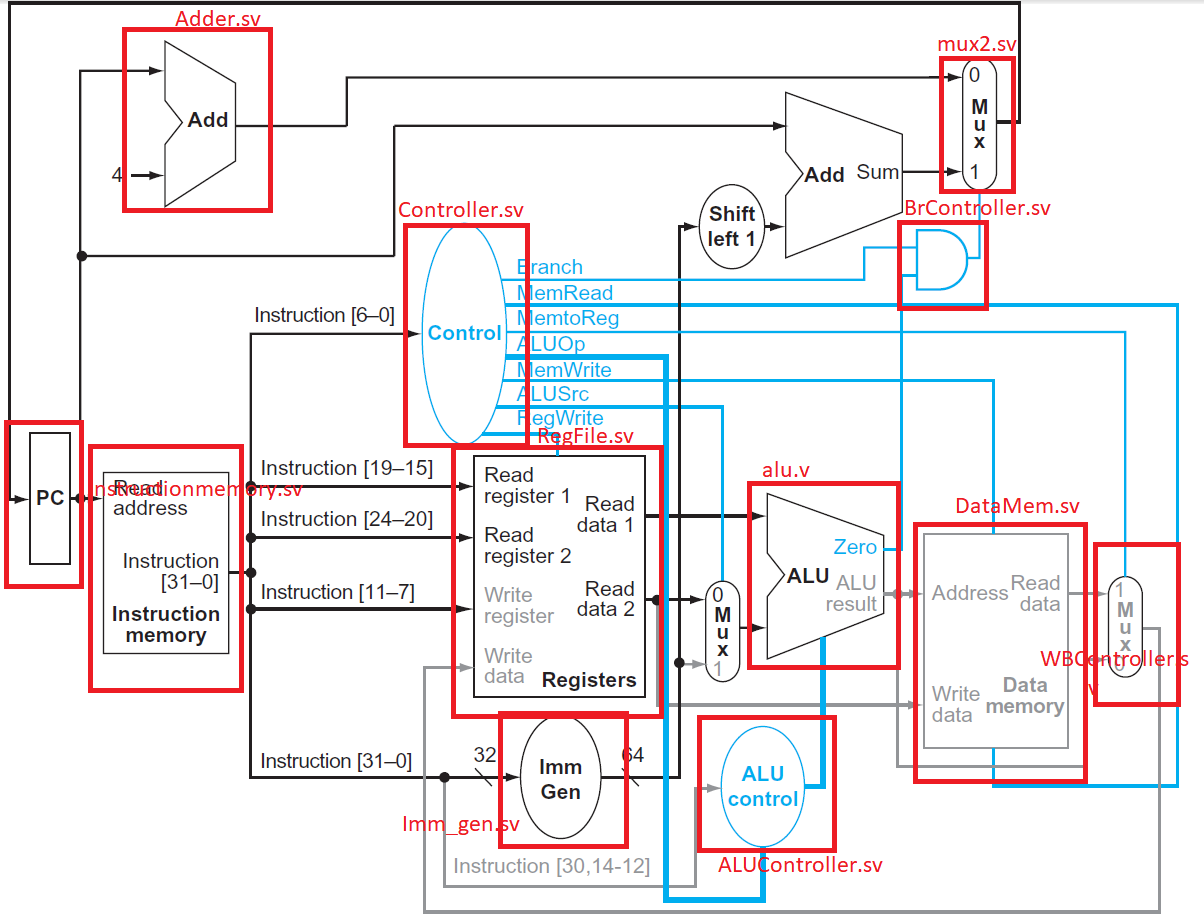
\includegraphics[width=1.0\textwidth]{block_-_Copy.PNG}
In the above diagram, the module outlined in red correspond to the files used to implement the Risc Processor.

\section{Wave Form}
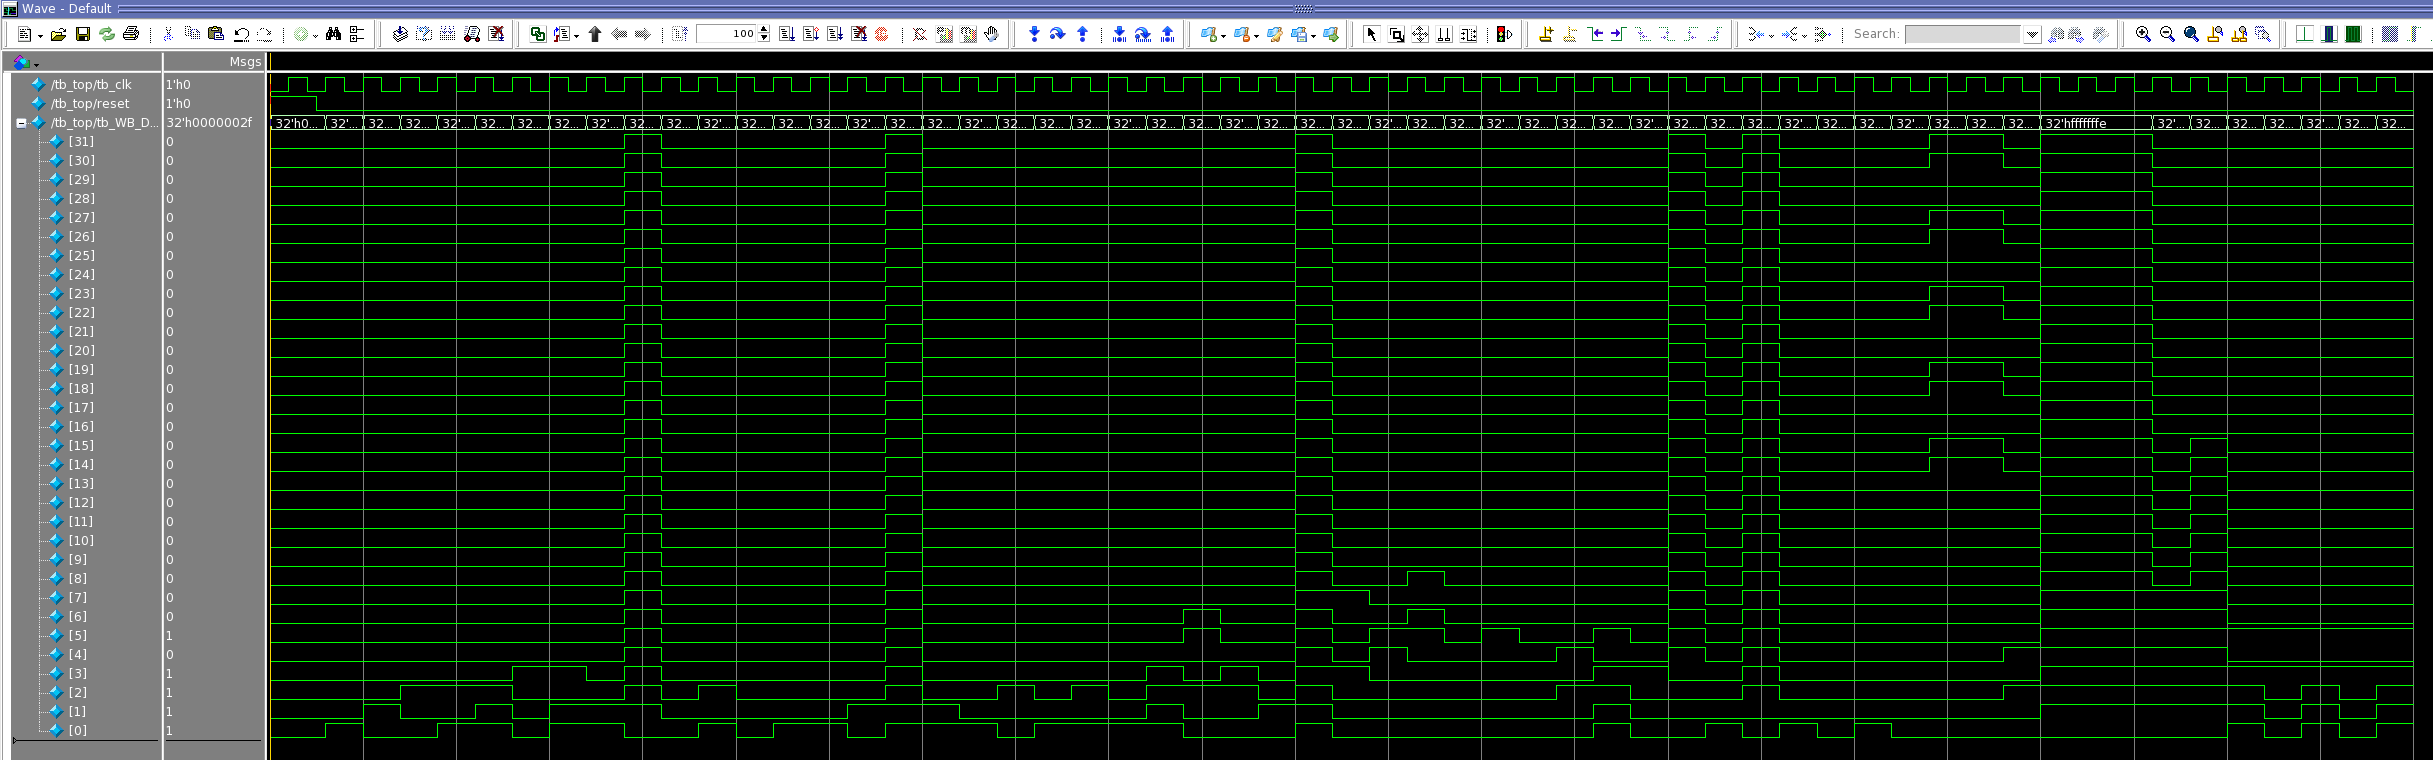
\includegraphics[width=1.0\textwidth]{wave2.PNG}
A snippet of the simulated waveform can be seen in the image above. Clk, reset, and ALU-Result are included in the wave.

\section{Synthesis Results}
\subsection{Clock/Time Report}
\begin{verbatim}
  Timing Path Group 'clk'
  -----------------------------------
  Levels of Logic:              34.00
  Critical Path Length:          5.53
  Critical Path Slack:          -3.56
  Critical Path Clk Period:      4.00
  Total Negative Slack:     -58235.06
  No. of Violating Paths:    17417.00
  Worst Hold Violation:          0.00
  Total Hold Violation:          0.00
  No. of Hold Violations:        0.00
  -----------------------------------
\end{verbatim}

The Critical path length and critical path slack are included in the above Clk report.

\subsection{Area Report}
\begin{verbatim}
  Area
  -----------------------------------
  Combinational Area:    88717.096124
  Noncombinational Area:
                        115255.832642
  Buf/Inv Area:           5739.334074
  Total Buffer Area:          3300.82
  Total Inverter Area:        2438.51
  Macro/Black Box Area:      0.000000
  Net Area:             168129.606231
  -----------------------------------
  Cell Area:            203972.928765
  Design Area:          372102.534996






\end{verbatim}

\subsection{Power Report}
\begin{verbatim}
Global Operating Voltage = 1.05 
Power-specific unit information :
    Voltage Units = 1V
    Capacitance Units = 1.000000ff
    Time Units = 1ns
    Dynamic Power Units = 1uW    (derived from V,C,T units)
    Leakage Power Units = 1pW


--------------------------------------------------------------------------------
                                       Switch   Int      Leak     Total
Hierarchy                              Power    Power    Power    Power    %
--------------------------------------------------------------------------------
riscv                                   128.452 2.79e+04 1.74e+11 2.02e+05 100.0
  dp (Datapath)                         127.146 2.79e+04 1.74e+11 2.02e+05 100.0
    data_mem (datamemory)                59.990 2.61e+04 1.60e+11 1.86e+05  92.1
    rf (RegFile)                         30.892 1.66e+03 1.08e+10 1.25e+04   6.2
    instr_mem (instructionmemory)         4.959    7.884 2.95e+08  307.352   0.2
1

\end{verbatim}

\end{document}